\documentclass[a4paper,twoside]{article}
\usepackage{graphicx}
\usepackage{url}
\usepackage{listings}
\usepackage{float}
\usepackage[width=0.89\textwidth]{caption}

\usepackage[natbib=true,
    style=numeric,
    sorting=none,
    backend=biber]{biblatex}
\addbibresource{o2bibliography.bib}

%\usepackage{lineno}
%\linenumbers

\def\O2{O$^2$}

\begin{document}

\title{ALICE \O2 data model proposal}

\author{Mikolaj Krzewicki \and Sylvain Chapeland \and Roberto Divia \and Matthias Richter \and David Rohr}
\date{
for the CWG4 data model group.\\[2ex]
\today
}

\maketitle

\abstract{This note presents a proposal for the ALICE \O2 data model. A base data layout and metadata format that allow for
efficient resource use are proposed. Application of the data model to online/offline data processing and quality control is discussed.}

\section{Introduction}

The ALICE online-offline (\O2) computing system \cite{o2tdr,o2} is a computing facility and a software framework designed for the processing of the ALICE data in the upcoming LHC Run 3.
The design aims at high data throughput and parallelism using a multiprocess model.
It does not, however, exclude the use of multithreading and other forms of concurrent processing inside of individual processes.

The data exchange between processes running within the \O2 system (called \O2 devices) is taken care of by the ALICE-FAIR (Alfa ) framework \cite{alfa}. Since this is the only communication mechanism foreseen for data exchange, it effectively serves the role of an API between the devices.
The Alfa framework provides data transport and synchronisation primitives via the FairMQ message queue library. FairMQ messages consist of raw memory buffers which are asynchronously queued and atomically delivered.

The data processed by the \O2 system consists of a set of data buffers originating from the detector hardware and the processing devices. The data fragments are logically grouped into (sub-) time frames. A (sub-) time frame contains the data associated to a period of data taking (typically several tens of ms, as dictated by the heartbeat trigger \cite{O2readout}) and/or the results of the processing of these data. In addition any data that might be necessary to describe and qualify the data set can be added to the logical group.

In order to assure consistent navigation within a time frame, each data fragment is described by a small metadata block containing the information about the content type of the payload, origin and coding (serialization) method.
In addition, the metadata block can be extended by the processing devices with additional information without the need to modify the payload.

Since time frame data volume is expected to be of the order of tens of gigabytes, the data model must facilitate communication approaches that will minimize resource use, i.e. avoid unnecessary copies of data.

\section{Vectored IO}

Vectored IO (also referred to as scatter/gather IO) is an important feature when dealing with multiple data buffers as it allows, in principle, to avoid the cost associated with serializing data into a single IO buffer.
Vectored IO is provided in FairMQ in the form of multi-part messages. A multi-part message consists of multiple independent buffers and is delivered atomically as a whole while preserving the ordering of the buffers.

The multi-part approach, in addition to minimizing the resource strain associated with IO buffer construction, also by construction reduces the need for (re-)synchronisation and event building; data fragments once associated to a single time frame remain that way throughout the entire chain regardless of the networking topology. Another benefit is that additional data parts can be attached or removed by other processing devices without copy overhead at any point of the processing chain.

\section{\O2 Message structure}

The \O2 message consists of a sequence of metadata-payload pairs contained within a multi-part message. Each payload is described by metadata contained in a separate message part. Since FairMQ preserves the ordering of the parts, the natural choice is to precede each data part with the associated metadata part in the message, as illustrated in figure \ref{fig:o2message}. 

\begin{figure}[h]
  \centering
  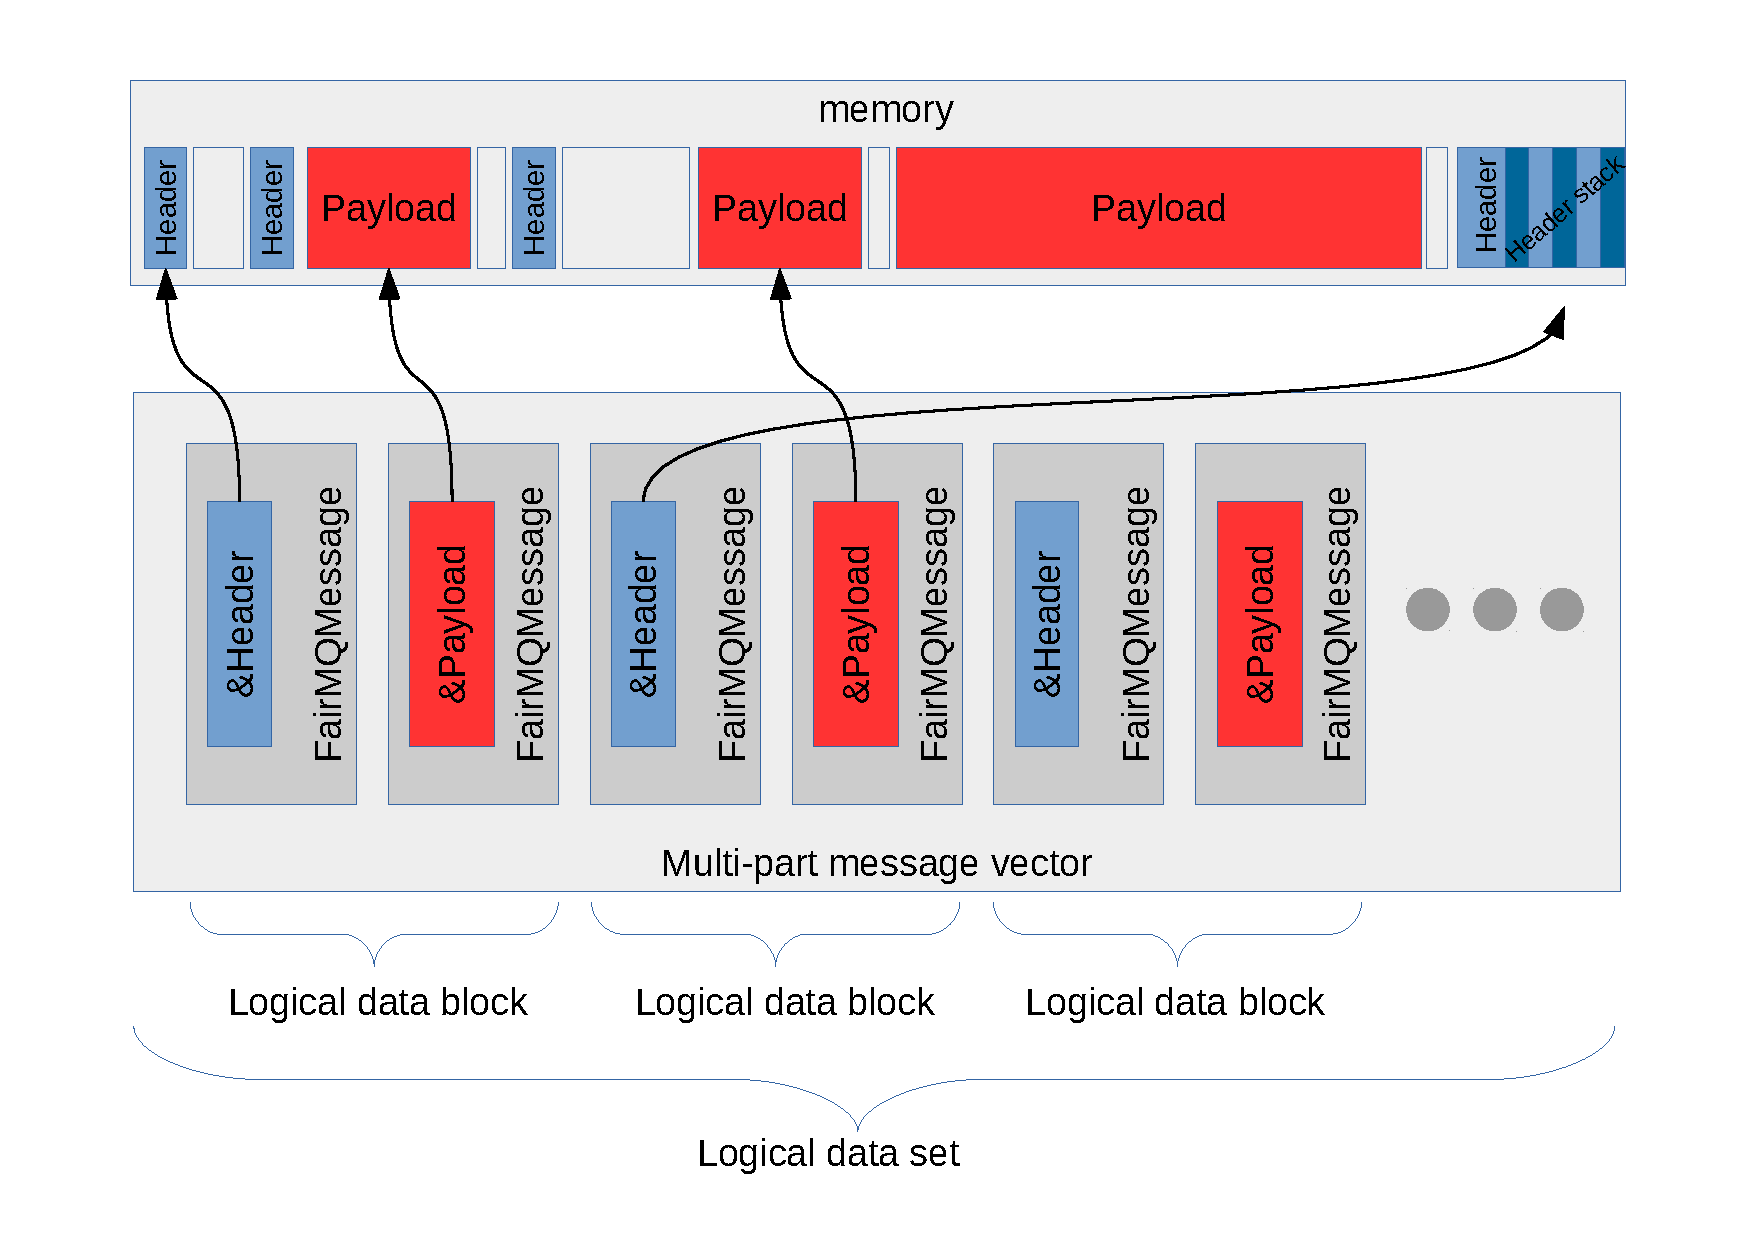
\includegraphics[width=0.89\textwidth]{multipartO2message.pdf}
  \caption{The \O2 message structure. Logical data blocks consisting of payload and metadata parts are contained in a multi-part FairMQ message (bottom). The buffers associated to the message parts do not have to be continuous in memory (top).}
  \label{fig:o2message} 
\end{figure}

Storing the metadata in separate buffers offers several advantages:

\begin{itemize}
  \item Since the metadata is separated from the payload already at transport level, efficient navigation is possible as only the (small) metadata parts need to be inspected.
  \item The size of the metadata buffer is not fixed enabling a scheme with flexible metadata content.
  \item The content of the data buffers, once produced by the hardware or a processing device, is immutable to other devices. Since the metadata is encapsulated in a separate buffer, it becomes possible to add additional information to the metadata with minimal cost and without modifying the payload downstream from the data producer.
\end{itemize}

\section{Metadata format}

The O2 metadata consists of a contiguous buffer containing a sequence of headers (header stack).
The byte representation of a header consists of a user defined body following a BaseHeader struct containing fields needed to:
\begin{itemize}
  \item Verify that the following data (header body) belongs to an \O2 header.
  \item Define the size of the entire header.
  \item Flag whether another header follows this one in the stack.
  \item Verify the version of the header.
  \item Signal the type of the header.
  \item Signal the packing/serialization scheme of the metadata body carried by the header.
\end{itemize}

The header stack should contain at least the standard DataHeader struct describing the basic payload properties. The DataHeader representation starts with the BaseHeader followed by bytes representing:
\begin{itemize}
  \item The functional data description uniquely determining the data type contained in the payload.
  \item The payload serialization method (e.g. ROOT, FlatBuffers, none) complementing the data description field.
  \item The origin of the data to identify the producer (e.g. detector system or a software subsystem).
  \item A data type dependent 64 bit specification. This can be used by the detectors to store e.g. the fine grained equipment ID like the link number for raw data or cluster finder instance for clusters\footnote{Based on HLT experience: most data types use some kind of fine grained ID. This field has been added here to avoid the overhead of a full header for what in most cases would be just one (64 bit) field.}.
  \item The payload buffer size\footnote{This is not strictly necessary online as the transport framework keeps track of the buffer sizes. Keeping this information is the header is useful for persistent storage and debugging purposes.}.
\end{itemize}

The memory layout of the BaseHeader and DataHeader structs and their interdependence is illustrated by the following code:

\lstset{language=C++
%,
%                keywordstyle=\color{blue},
%                stringstyle=\color{red},
%                commentstyle=\color{green},
%                morecomment=[l][\color{magenta}]{\#}
}
\begin{lstlisting}
struct BaseHeader
{
  uint32_t  magicStringInt;
  uint32_t  headerSize;
  uint32_t  flags;
  uint32_t  headerVersion;
  uint64_t  headerDescription;
  uint64_t  headerSerialization;
};

struct DataHeader : public BaseHeader
{
  uint64_t dataDescription[2];
  uint32_t dataOrigin;
  uint32_t reserved;
  uint64_t payloadSerializationMethod;
  uint64_t subSpecification;
  uint64_t payloadSize;
};

\end{lstlisting}



Other headers can be defined similarly to DataHeader and included in the header stack based on the requirements. Examples include trigger information for triggered detector data, object name for ROOT objects used in quality control etc.

\section{Data formats}

\section{Interfaces}

\printbibliography

\end{document}
